\section{PSoC 5 Applikationsmodel}

Alle diagrammer i dette kapitel er vedlagt som bilag i zip filen i mappen APPSoC da de kan være meget svære at læse efter at de er blevet skaleret ned til at passe i PDF filen, her kan der ligeledes findes et sekvensdiagram for hver af de 2 use-cases hvor der ikke benyttes ref-blokke til at simplificere dem.

\subsection{Sekvensdiagrammer der anvendes i Applikationsmodel for use-case 1 og 2}

Da sekvensdiagrammerne for use-case 1 og 2 er meget store er det opdelt i mindre bider for at gøre de overordnede diagrammer mere overskuelige, diagrammerne i dette afsnit vil blivere refereret til i de sekvensdiagrammer der anvendes til at beskrive use-case 1 og 2 i de følgende afsnit.

\begin{figure}[H]
	\caption{Sekvensdiagram for funktionen gå til position}
	\label{SD:PSoC:GaaTilPos}
	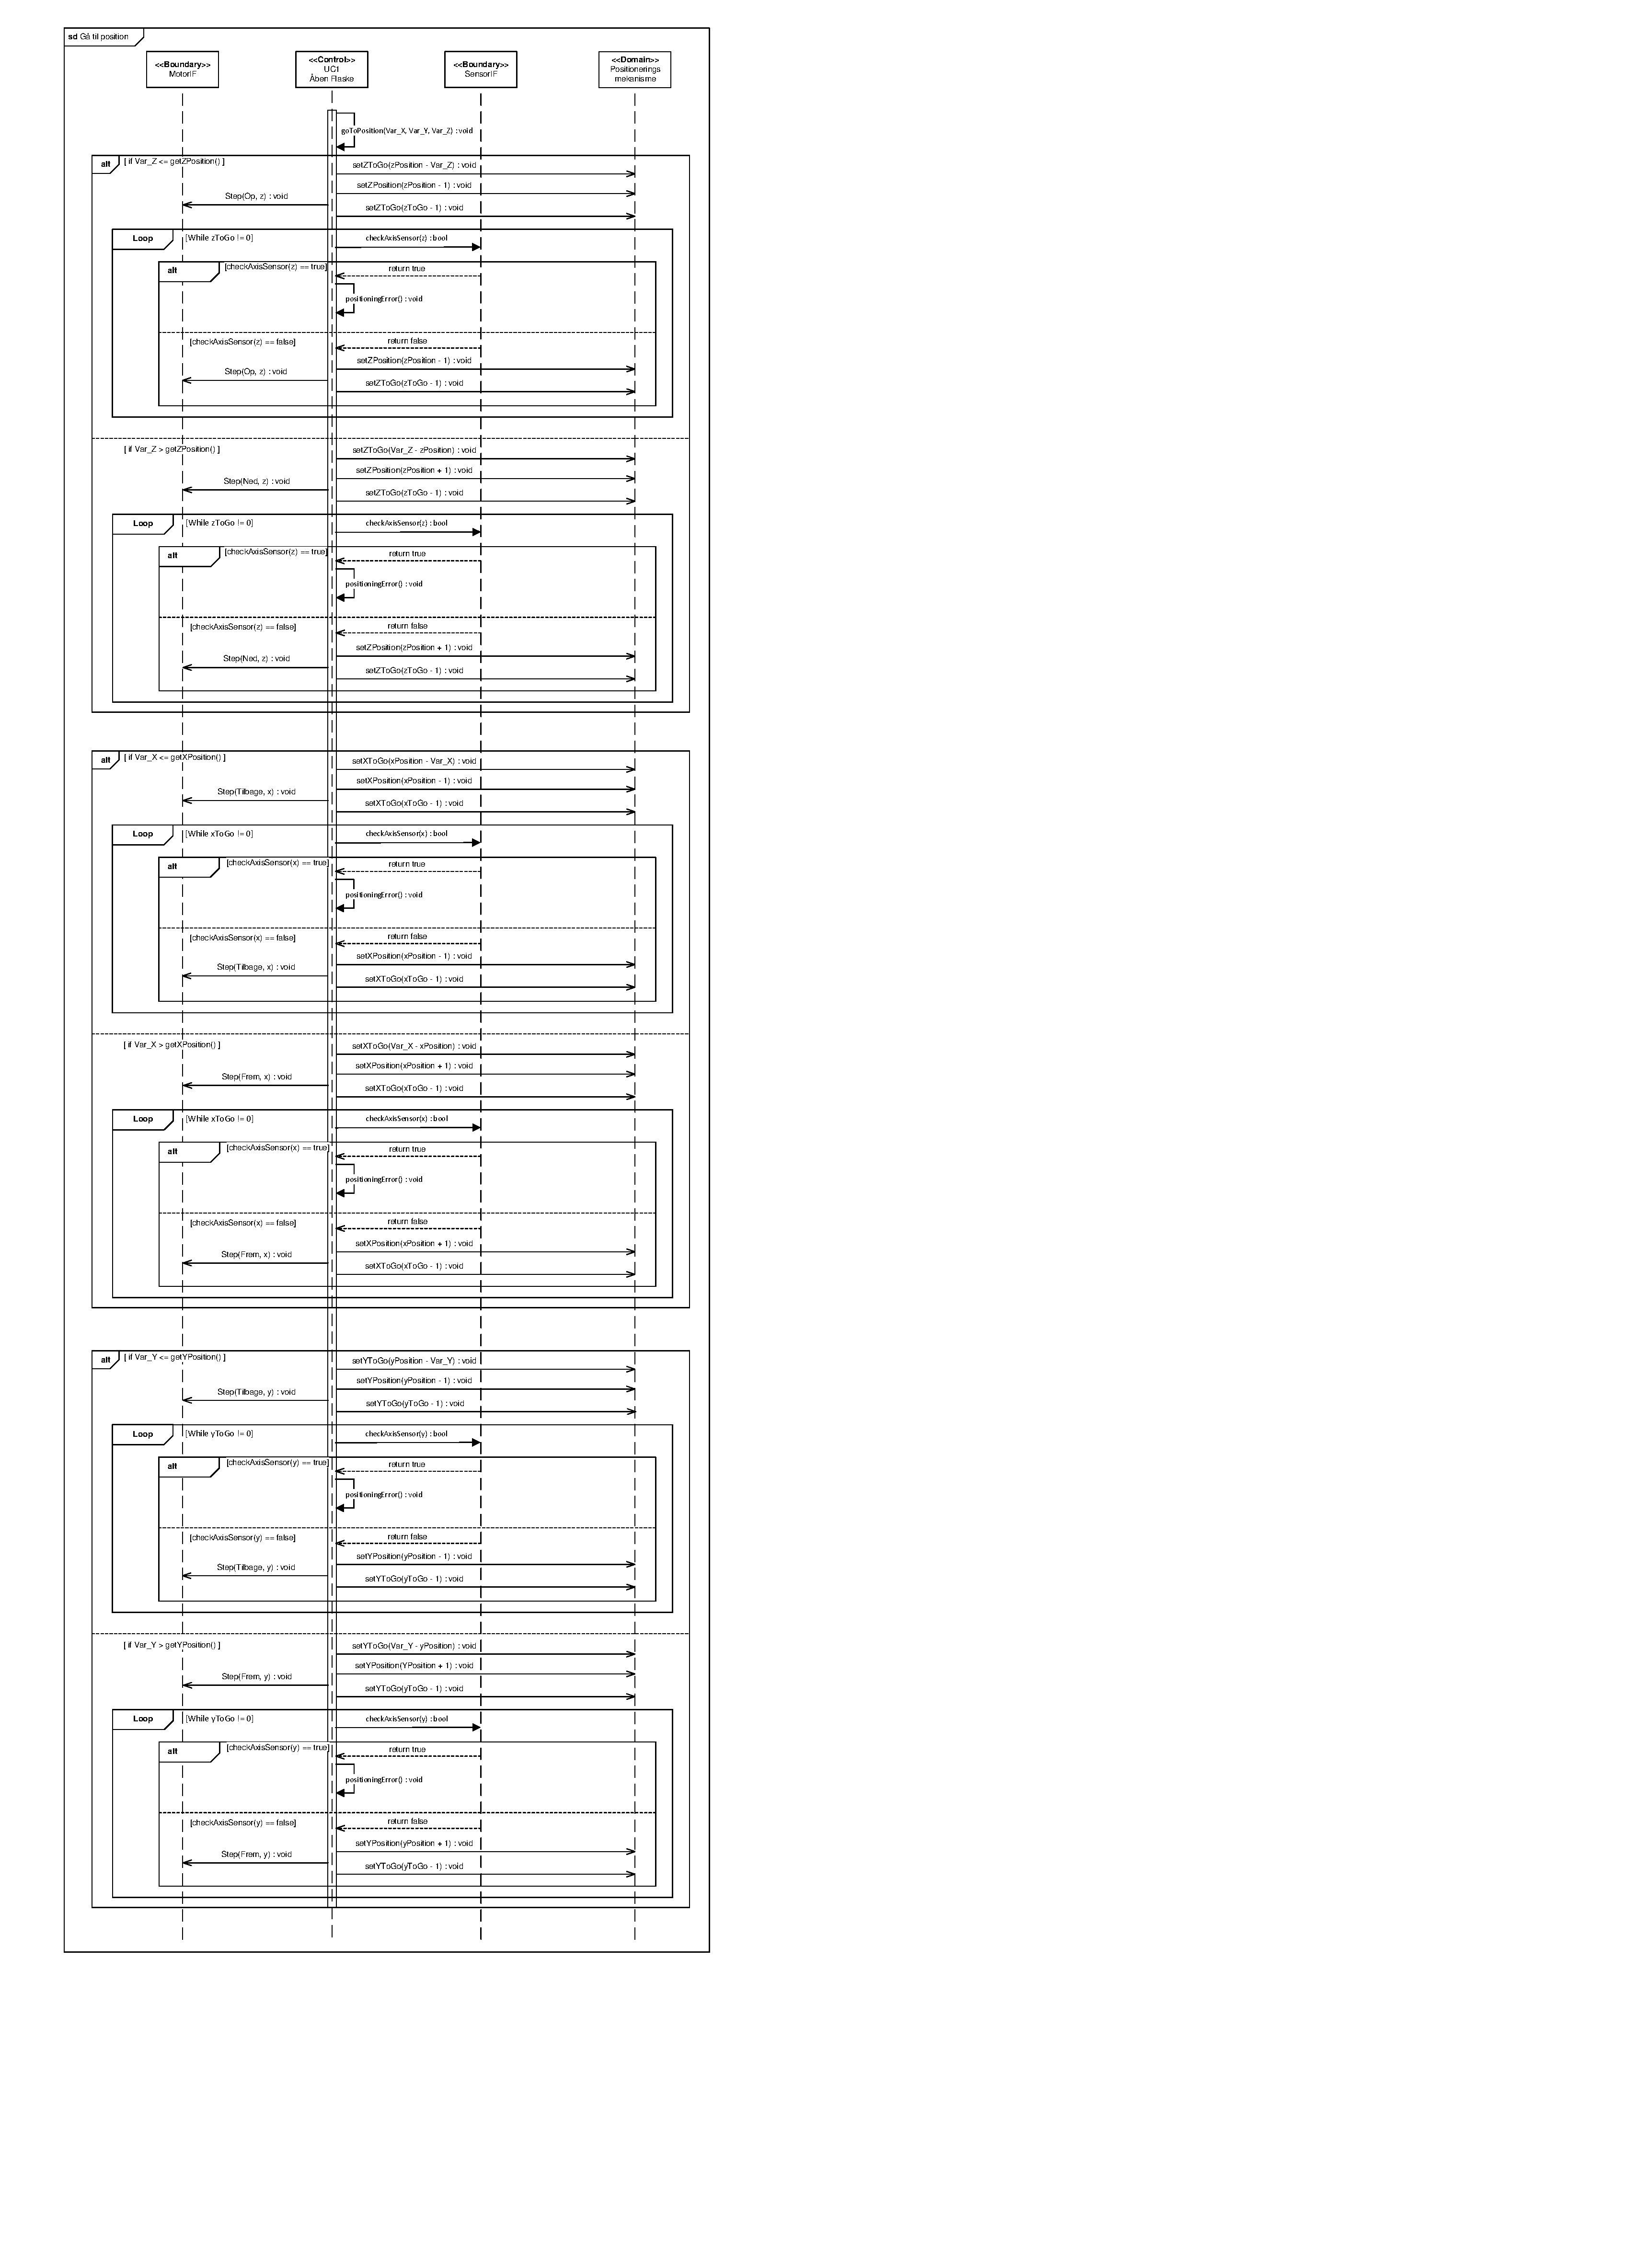
\includegraphics[scale=0.29,trim=0 0 1000 0]{APPSoC/SD-Gaa-til-position-v1}
\end{figure}

\begin{figure}[H]
	\caption{Sekvensdiagram for funktionen Scan x aksen}
	\label{SD:PSoC:ScanX}
	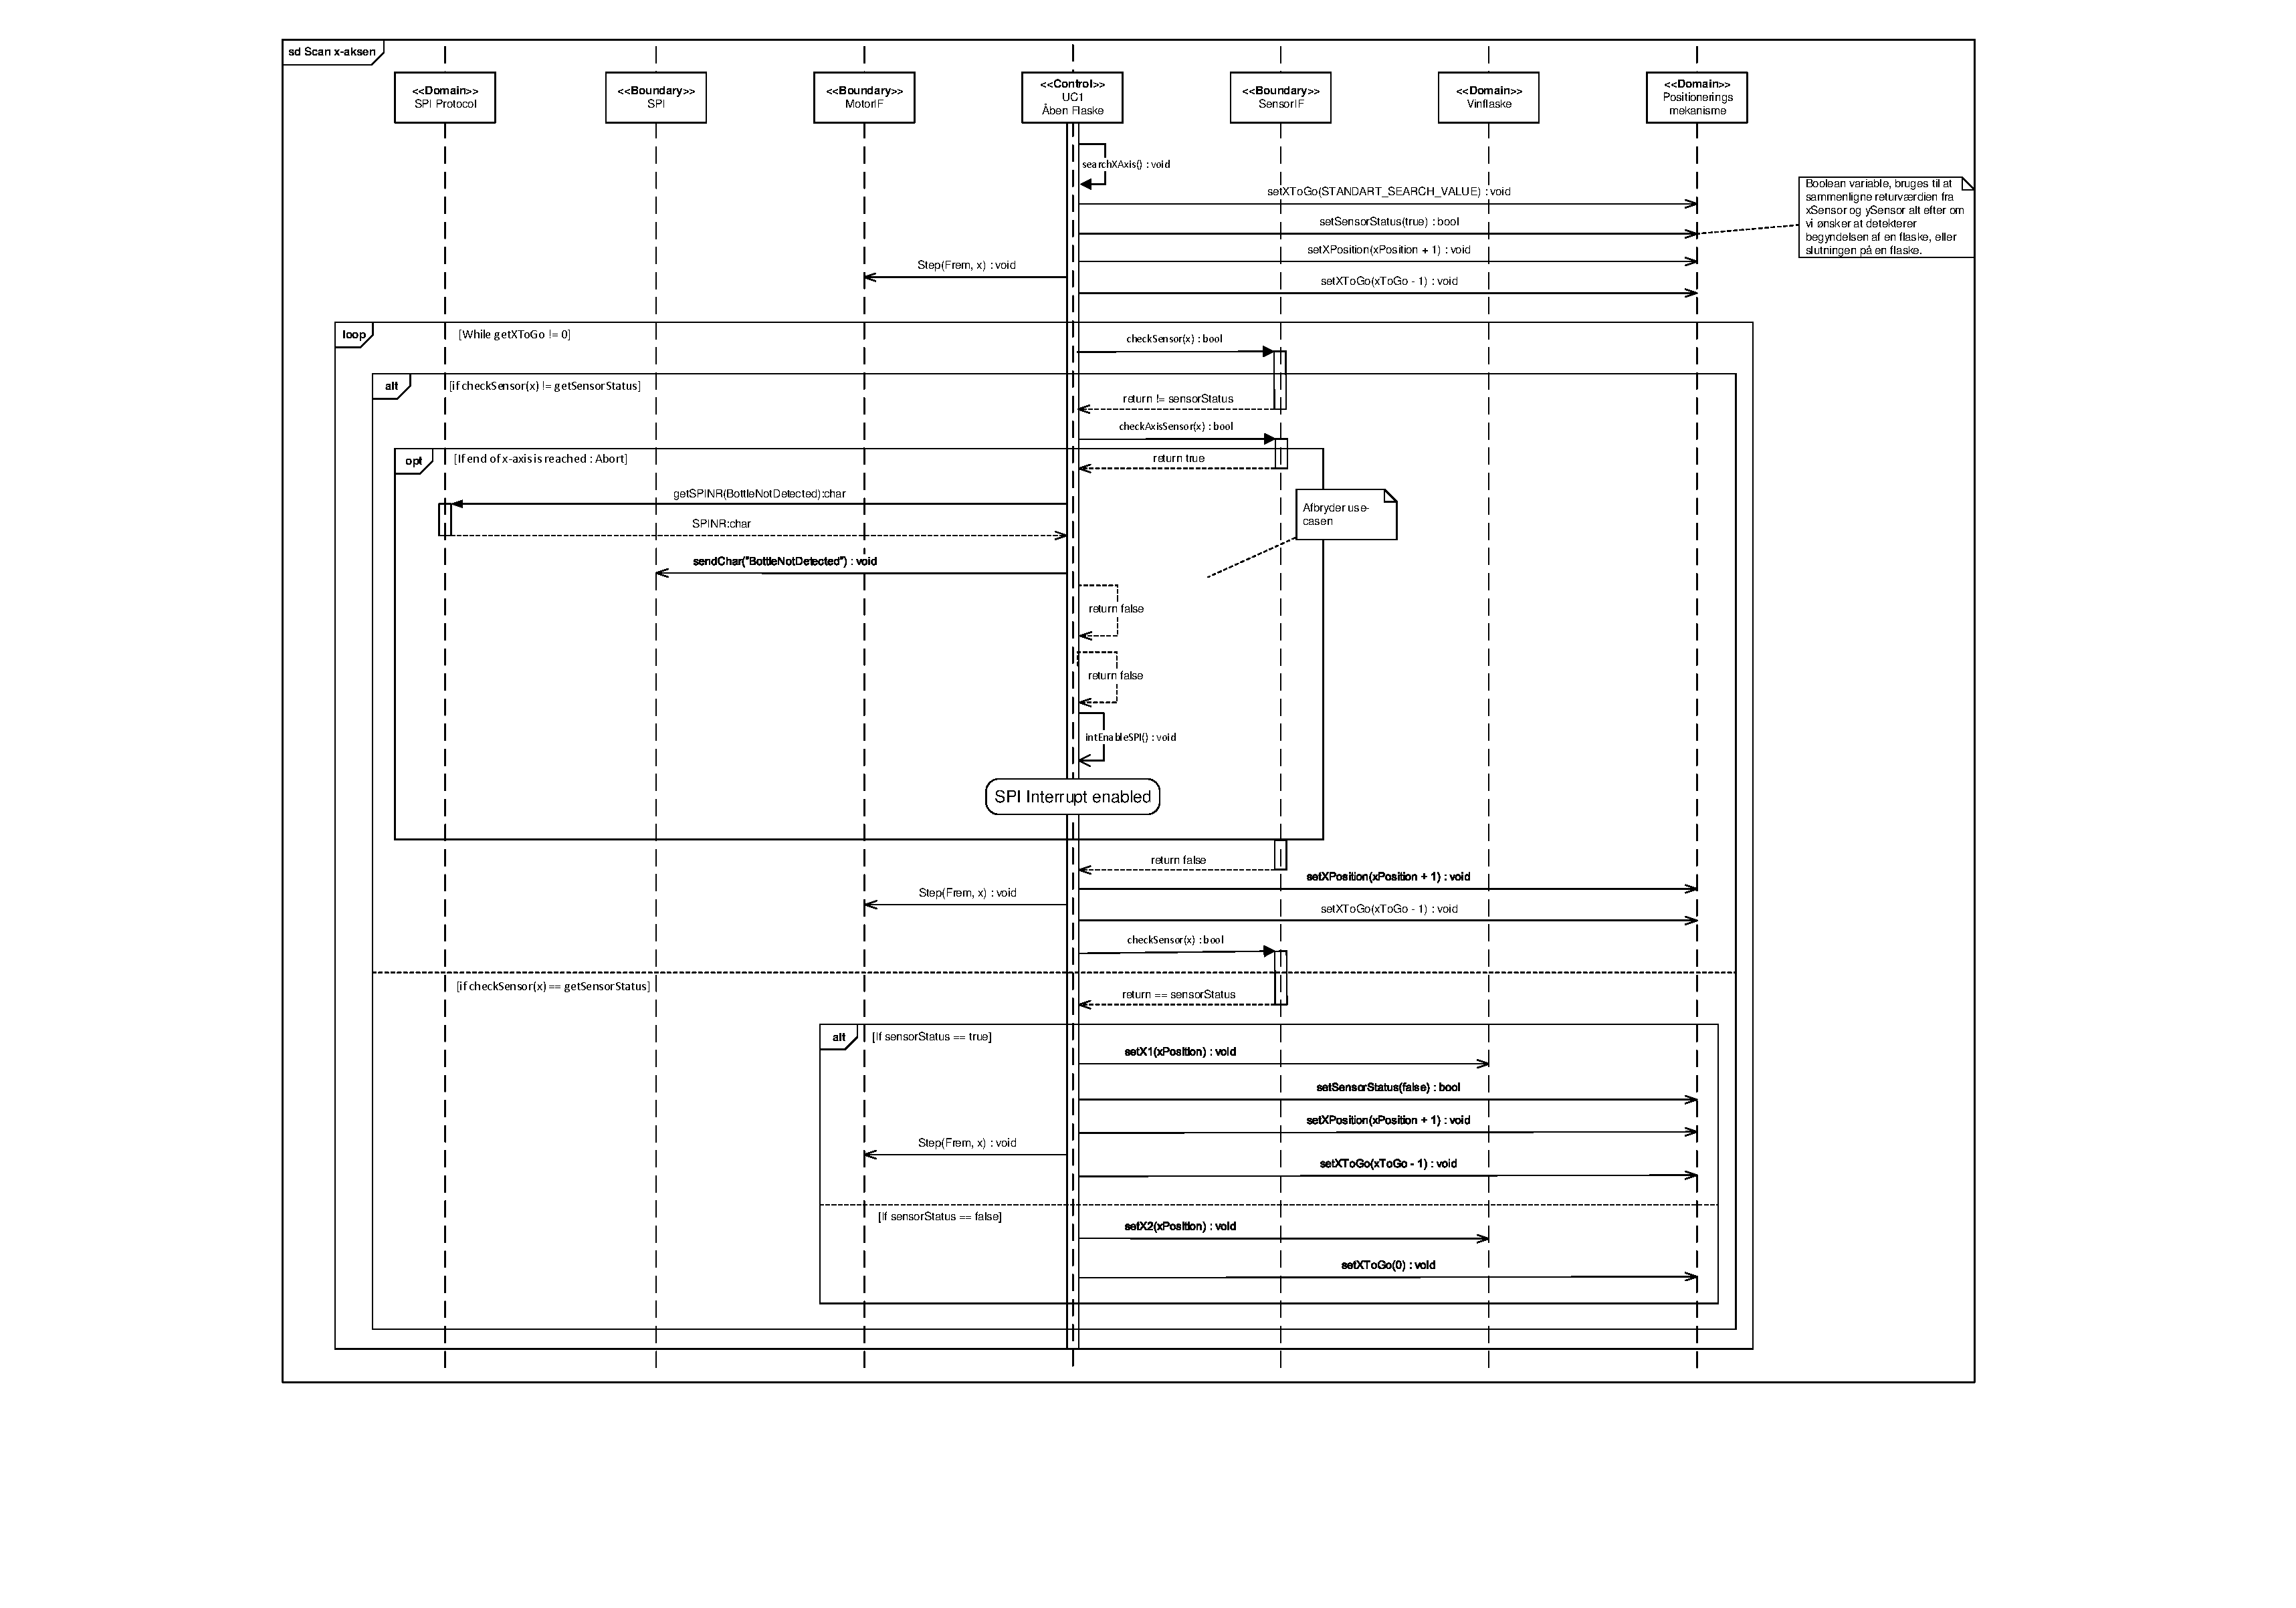
\includegraphics[scale=0.29,trim=200 150 0 0, clip]{APPSoC/SD-Scan-x-aksen}
\end{figure}

\begin{figure}[H]
	\caption{Sekvensdiagram for funktionen Scan y aksen}
	\label{SD:PSoC:ScanY}
	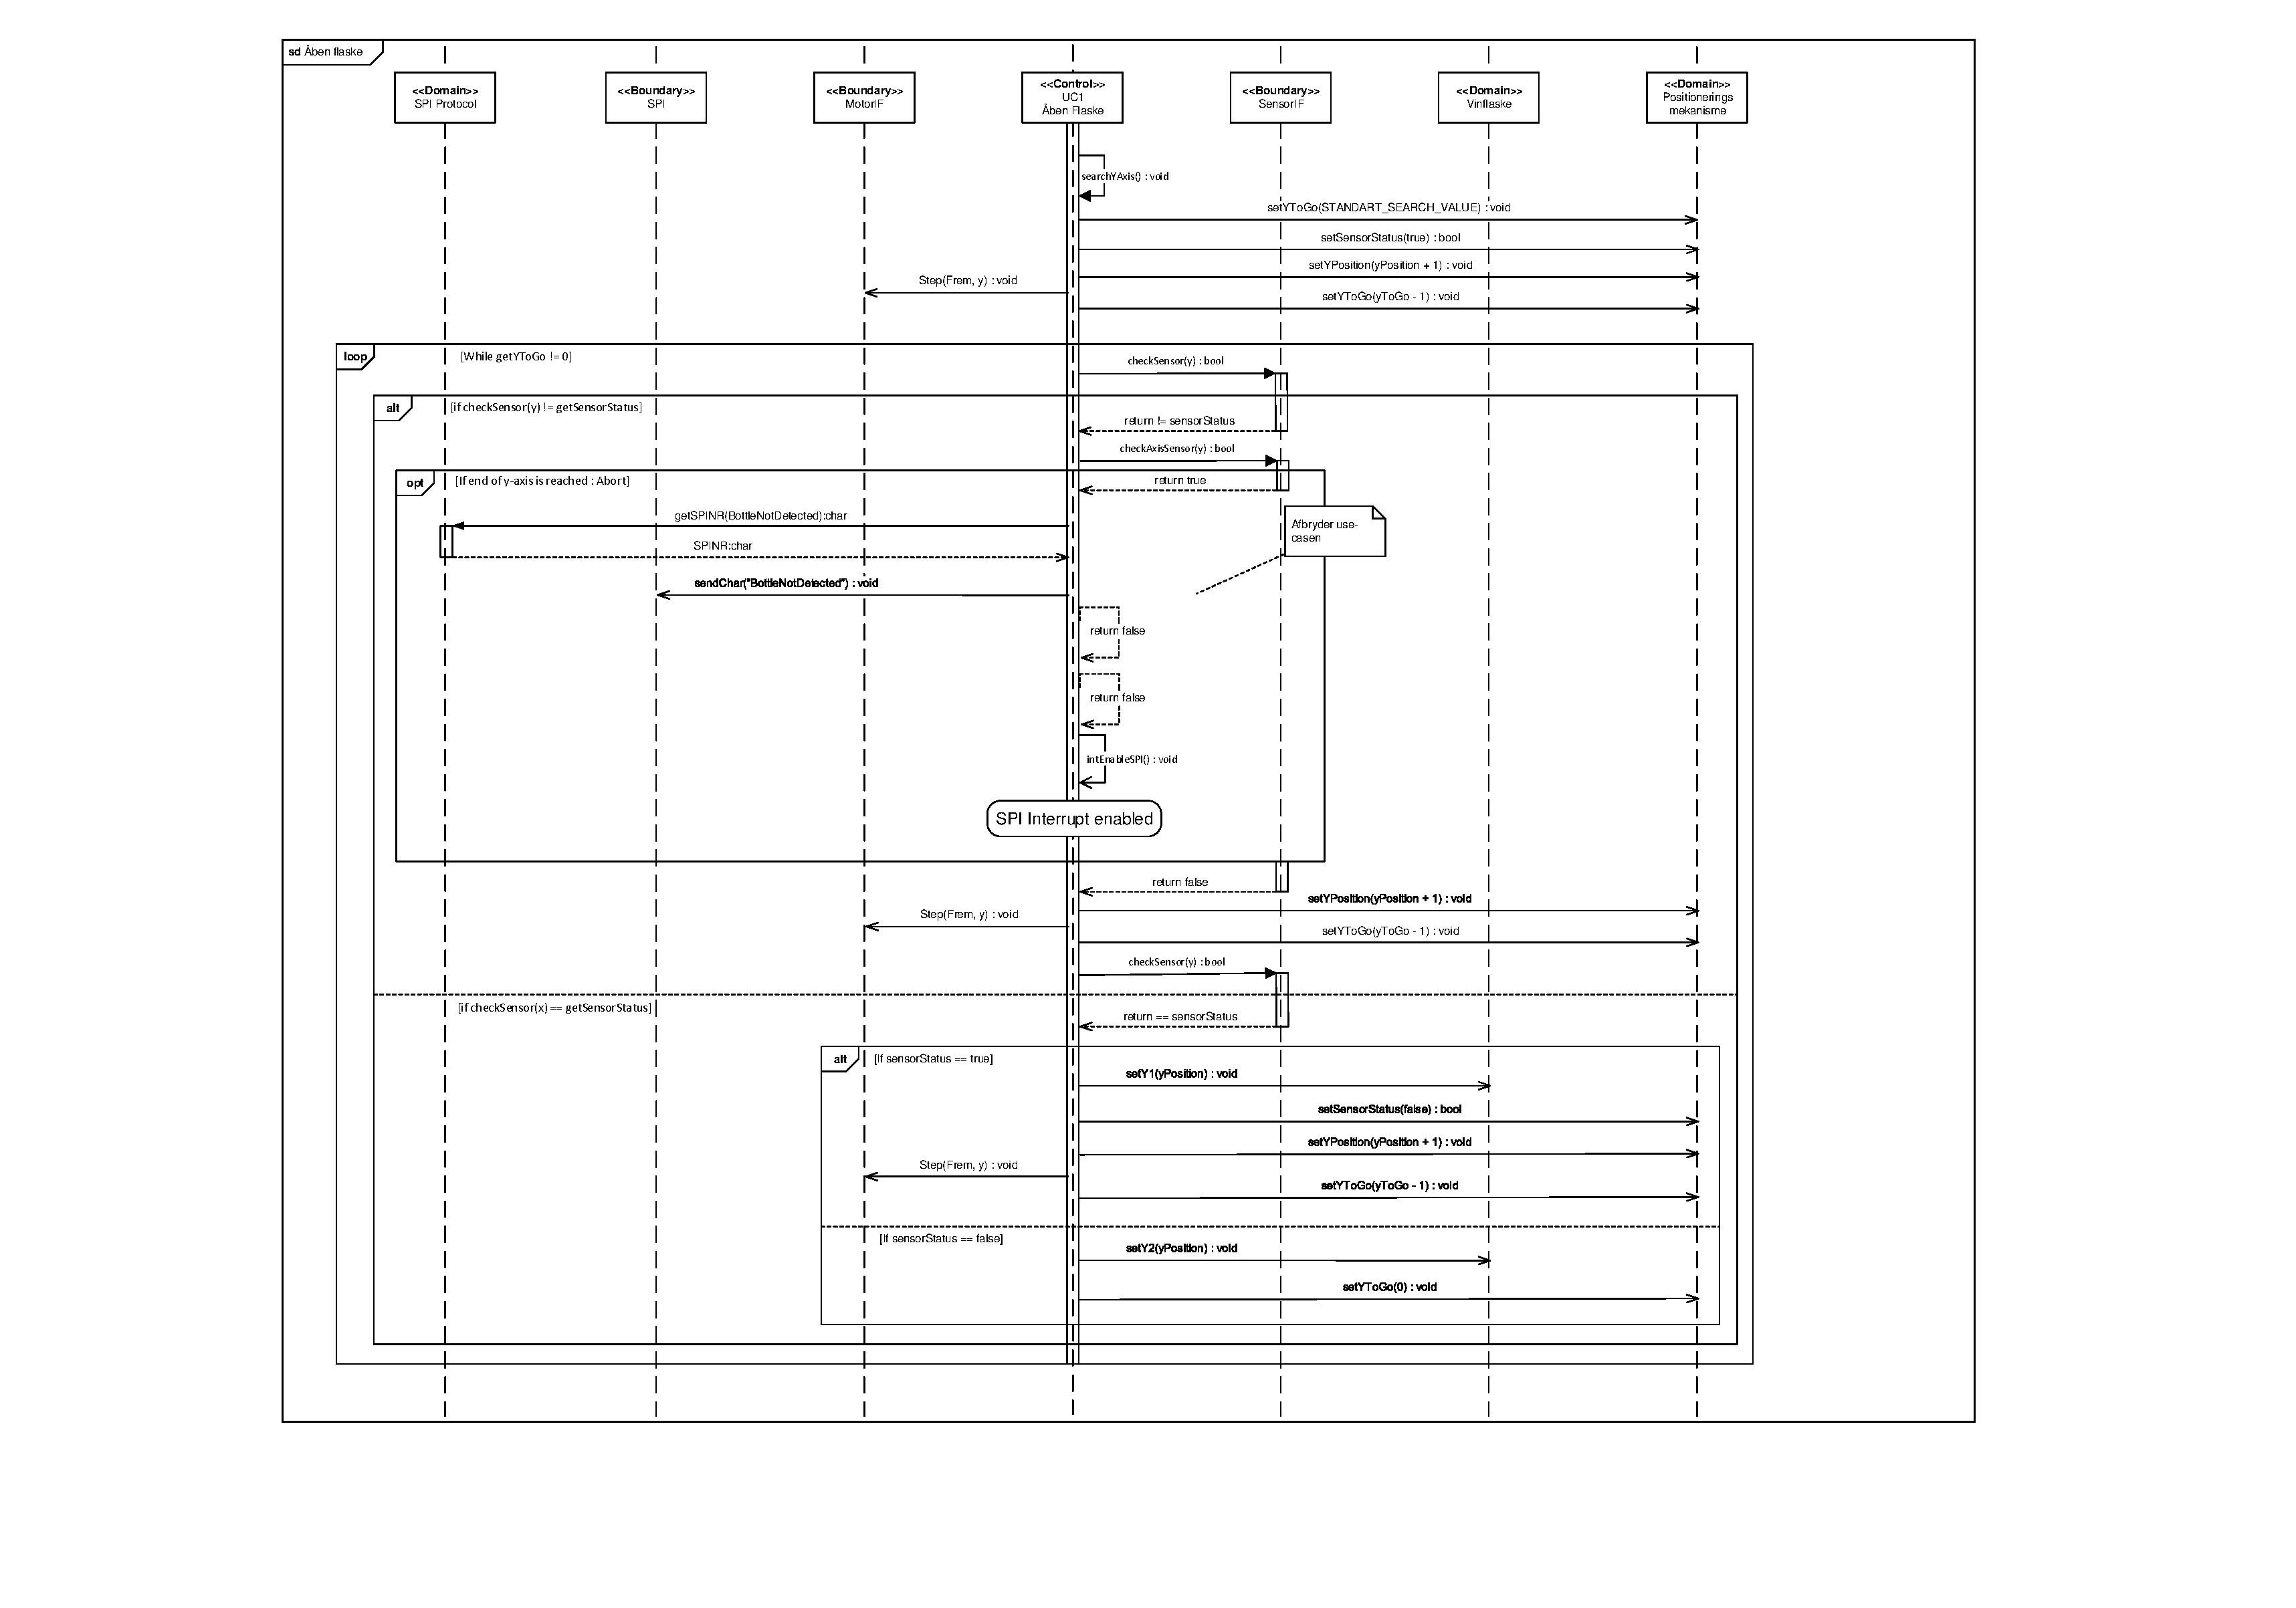
\includegraphics[scale=0.29,trim=200 100 0 0,clip]{APPSoC/SD-Scan-y-aksen}
\end{figure}

\begin{figure}[H]
	\caption{Sekvensdiagram for funktionen Scan z aksen}
	\label{SD:PSoC:ScanZ}
	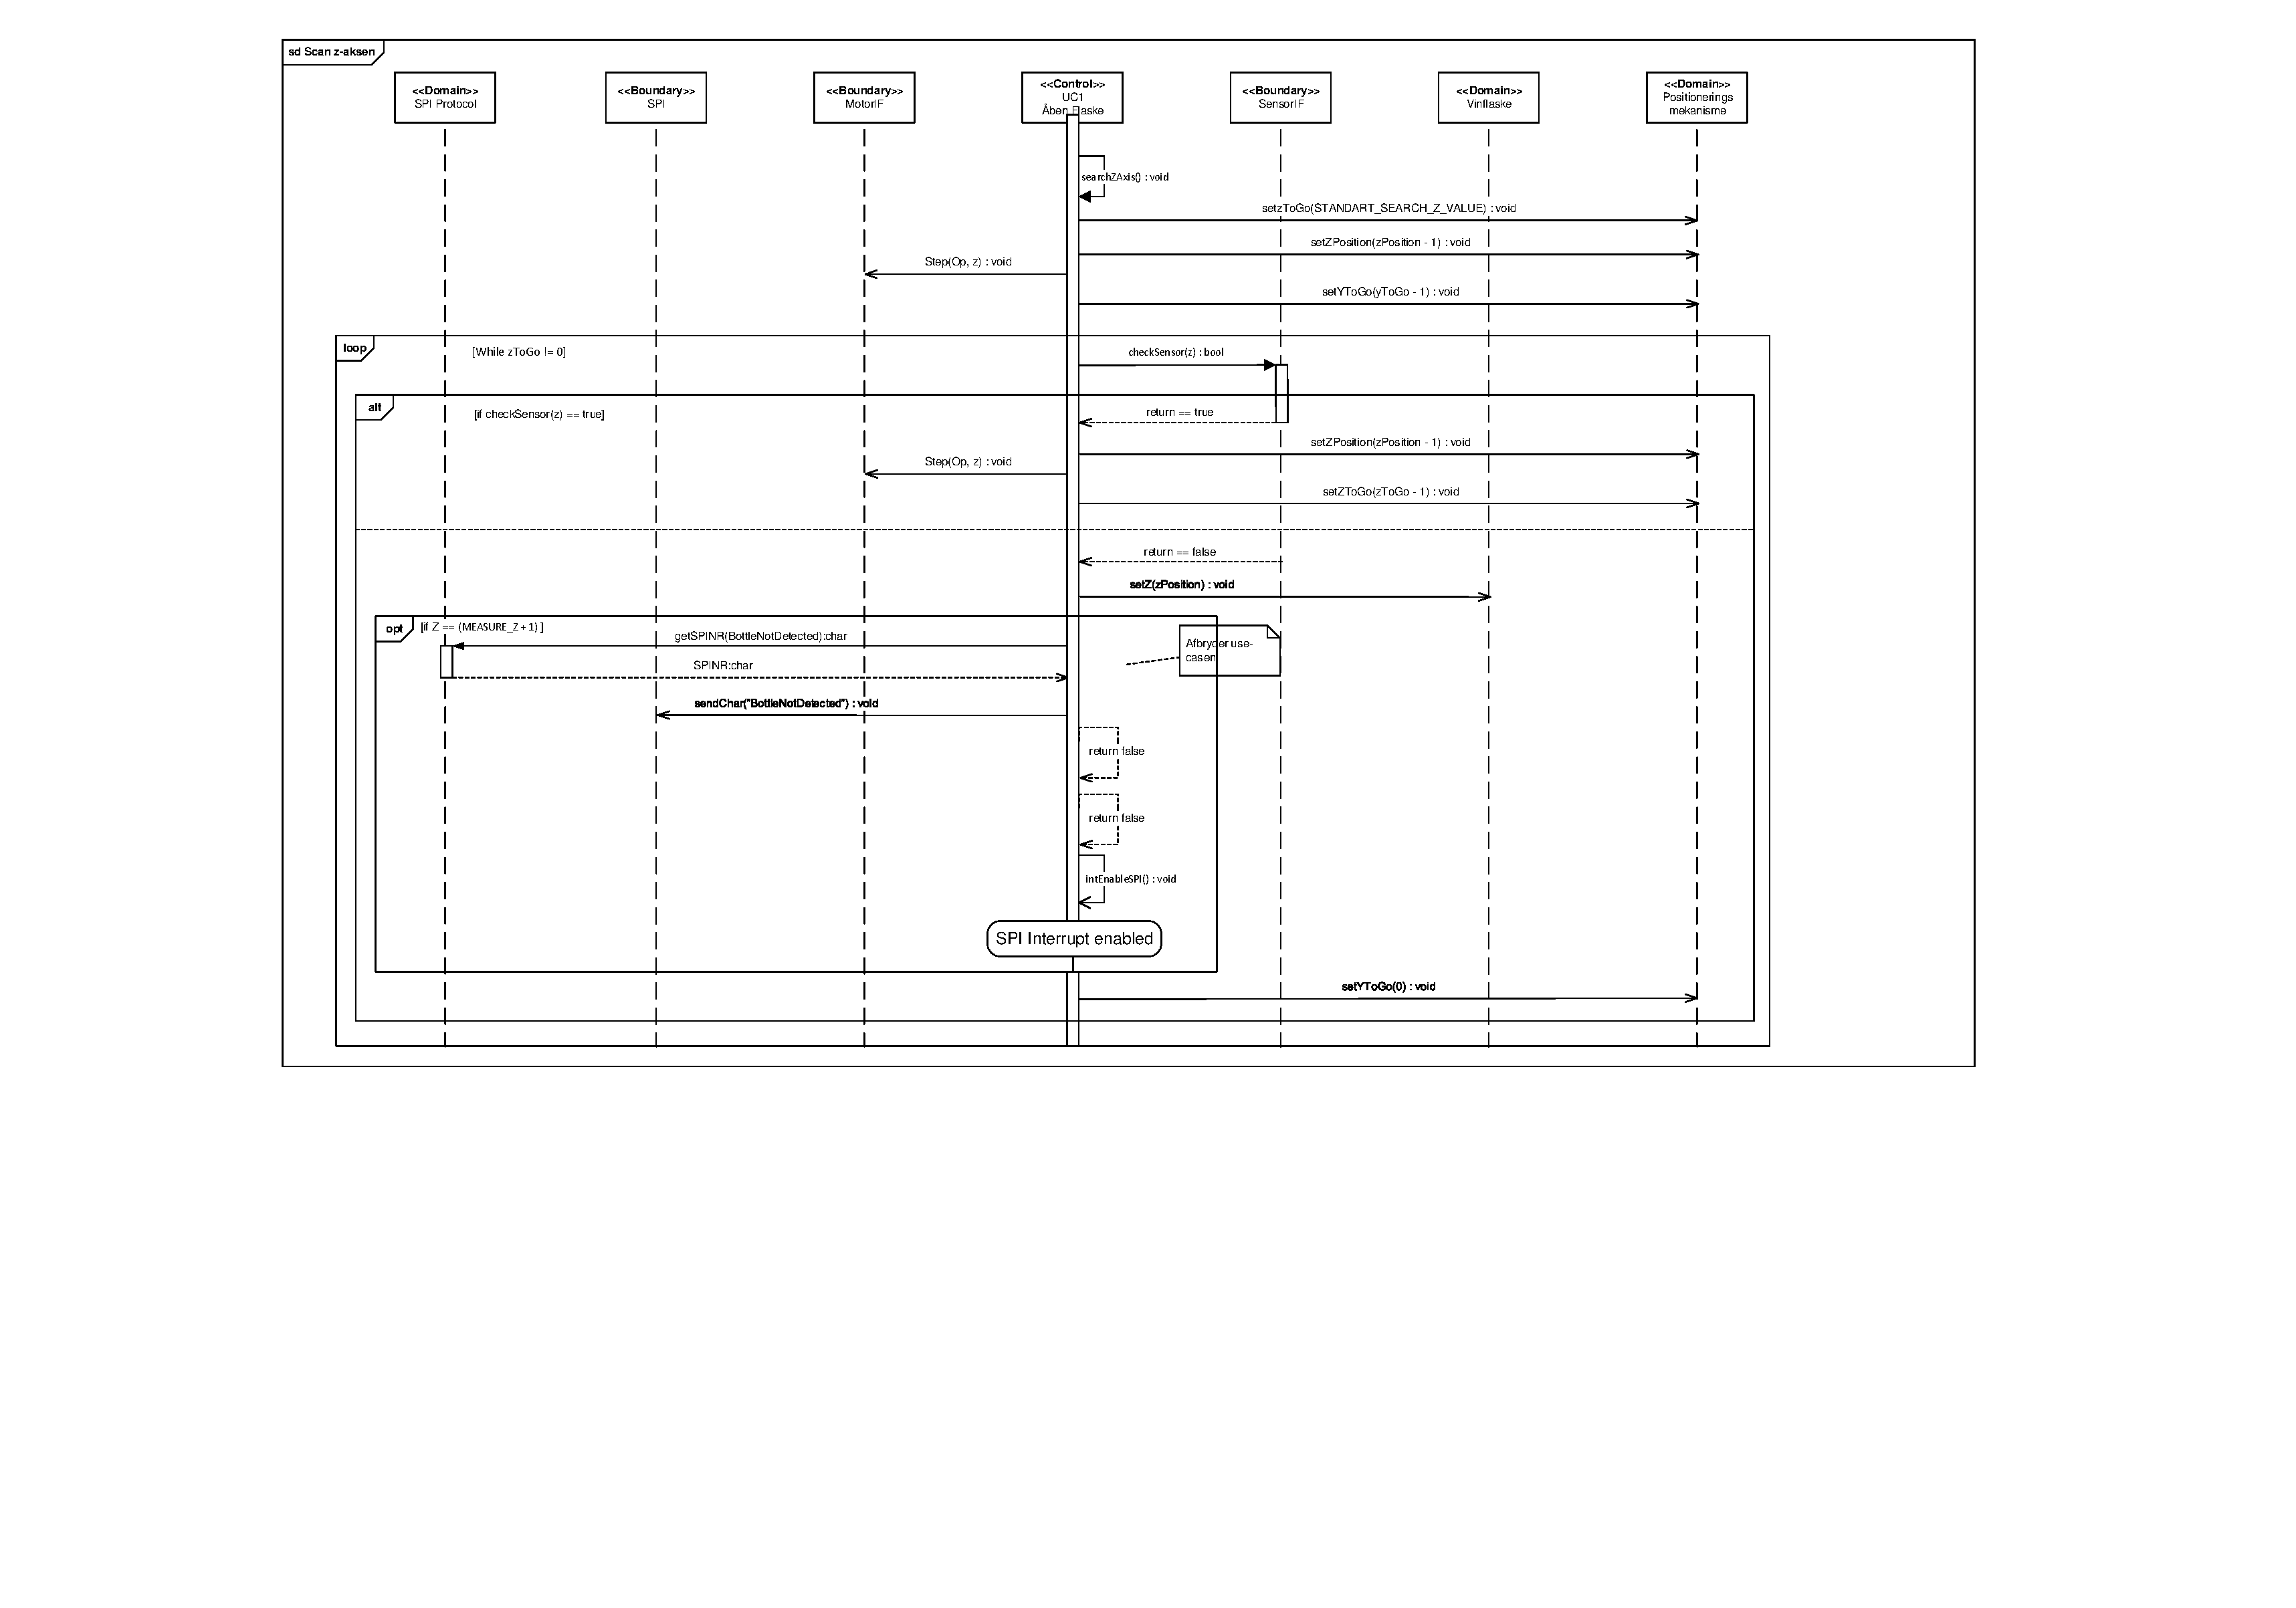
\includegraphics[scale=0.29,trim=200 100 0 0, clip]{APPSoC/SD-Scan-z-aksen}
\end{figure}

\subsection{Applikationsmodel for use-case 1}

\begin{figure}[H]
	\caption{Sekvensdiagram for use-case 1: åbn nu}
	\label{SD:PSoC:UC1}
	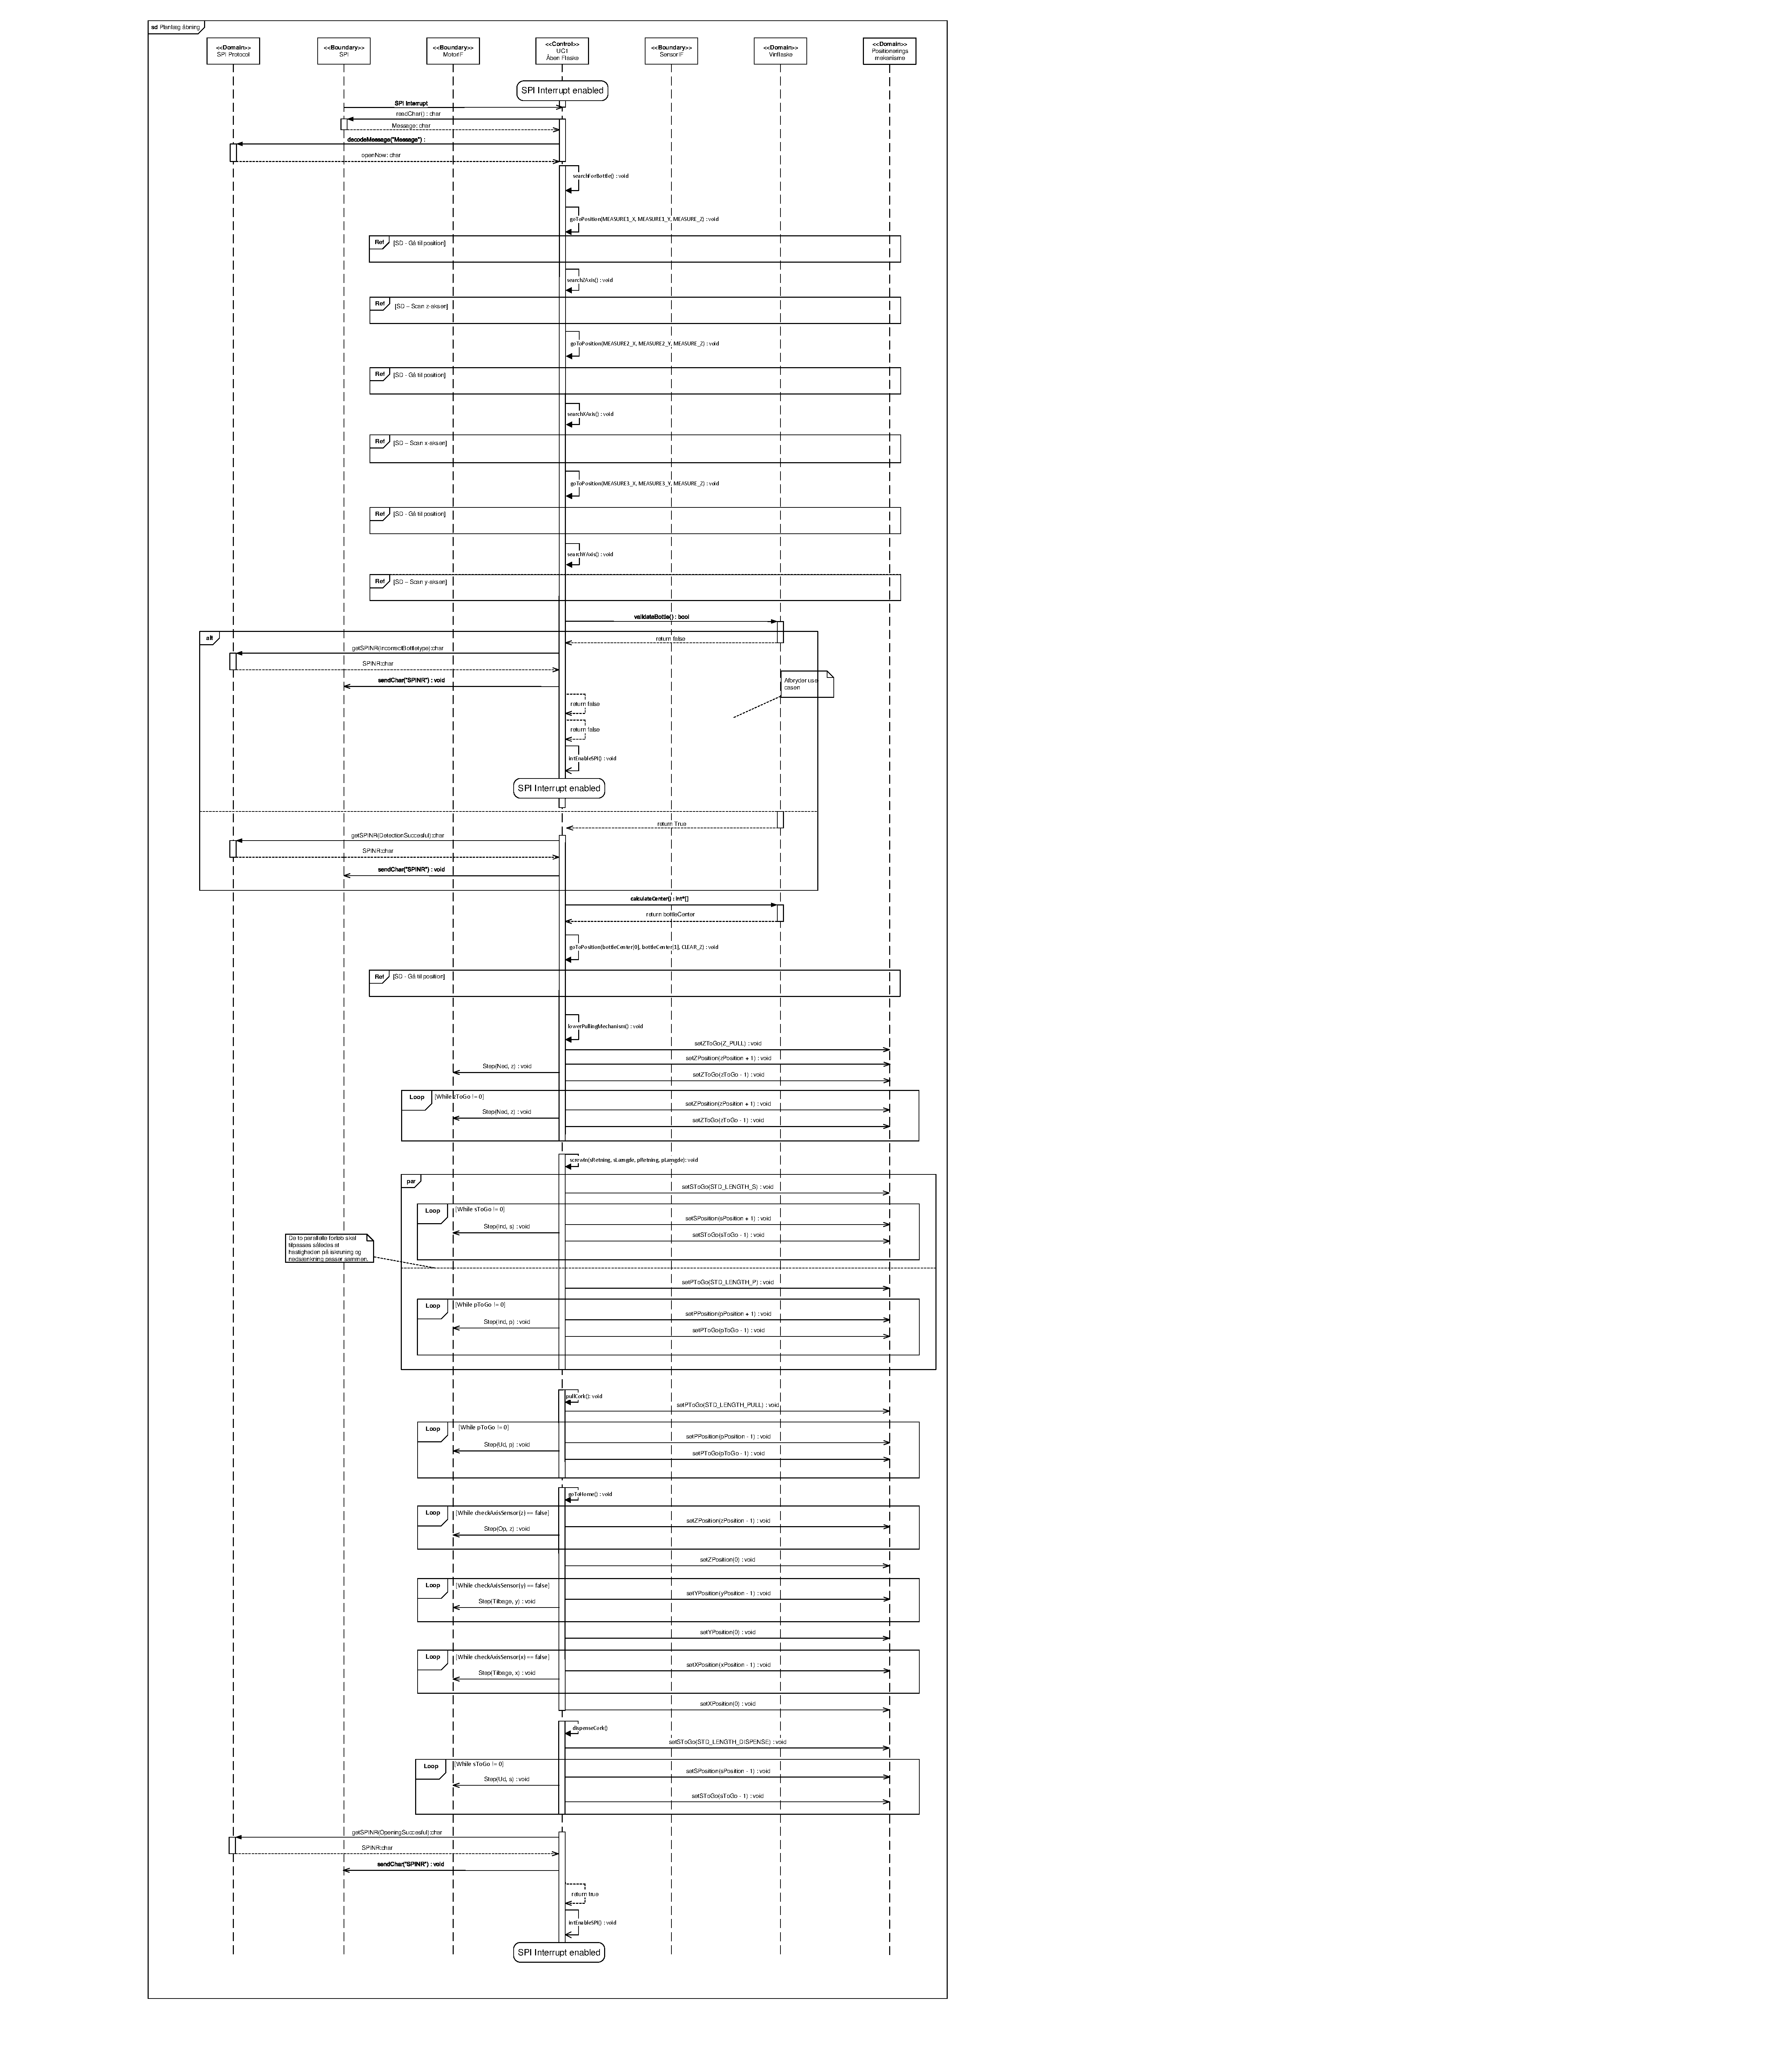
\includegraphics[scale=0.2,trim=0 0 0 0, clip]{APPSoC/UC1-Aaben-nu-v1-simplified}
\end{figure}

Ud fra sekvensdiagrammet på figur \ref{SD:PSoC:UC1} side \pageref{SD:PSoC:UC1} samt sekvensdiagrammerne sektionen "Sekvensdiagrammer der anvendes i Applikationsmodel for use-case 1 og 2" er der udført metodeidentifikation hvilket har resulteret i klassediagrammet på figur \ref{CD:PSoC:UC1} side \pageref{CD:PSoC:UC1}.

\begin{figure}[H]
	\caption{Klassediagram for use-case 1: åbn nu}
	\label{CD:PSoC:UC1}
	\includegraphics[scale=0.35,trim=0 0 0 0, clip]{APPSoC/UC1-CD-Aaben-nu-PSoC}
\end{figure}

\subsection{Applikationsmodel for use-case 2}


\begin{figure}[H]
	\caption{Sekvensdiagram for use-case 2: Planlæg åbning}
	\label{SD:PSoC:UC2}
	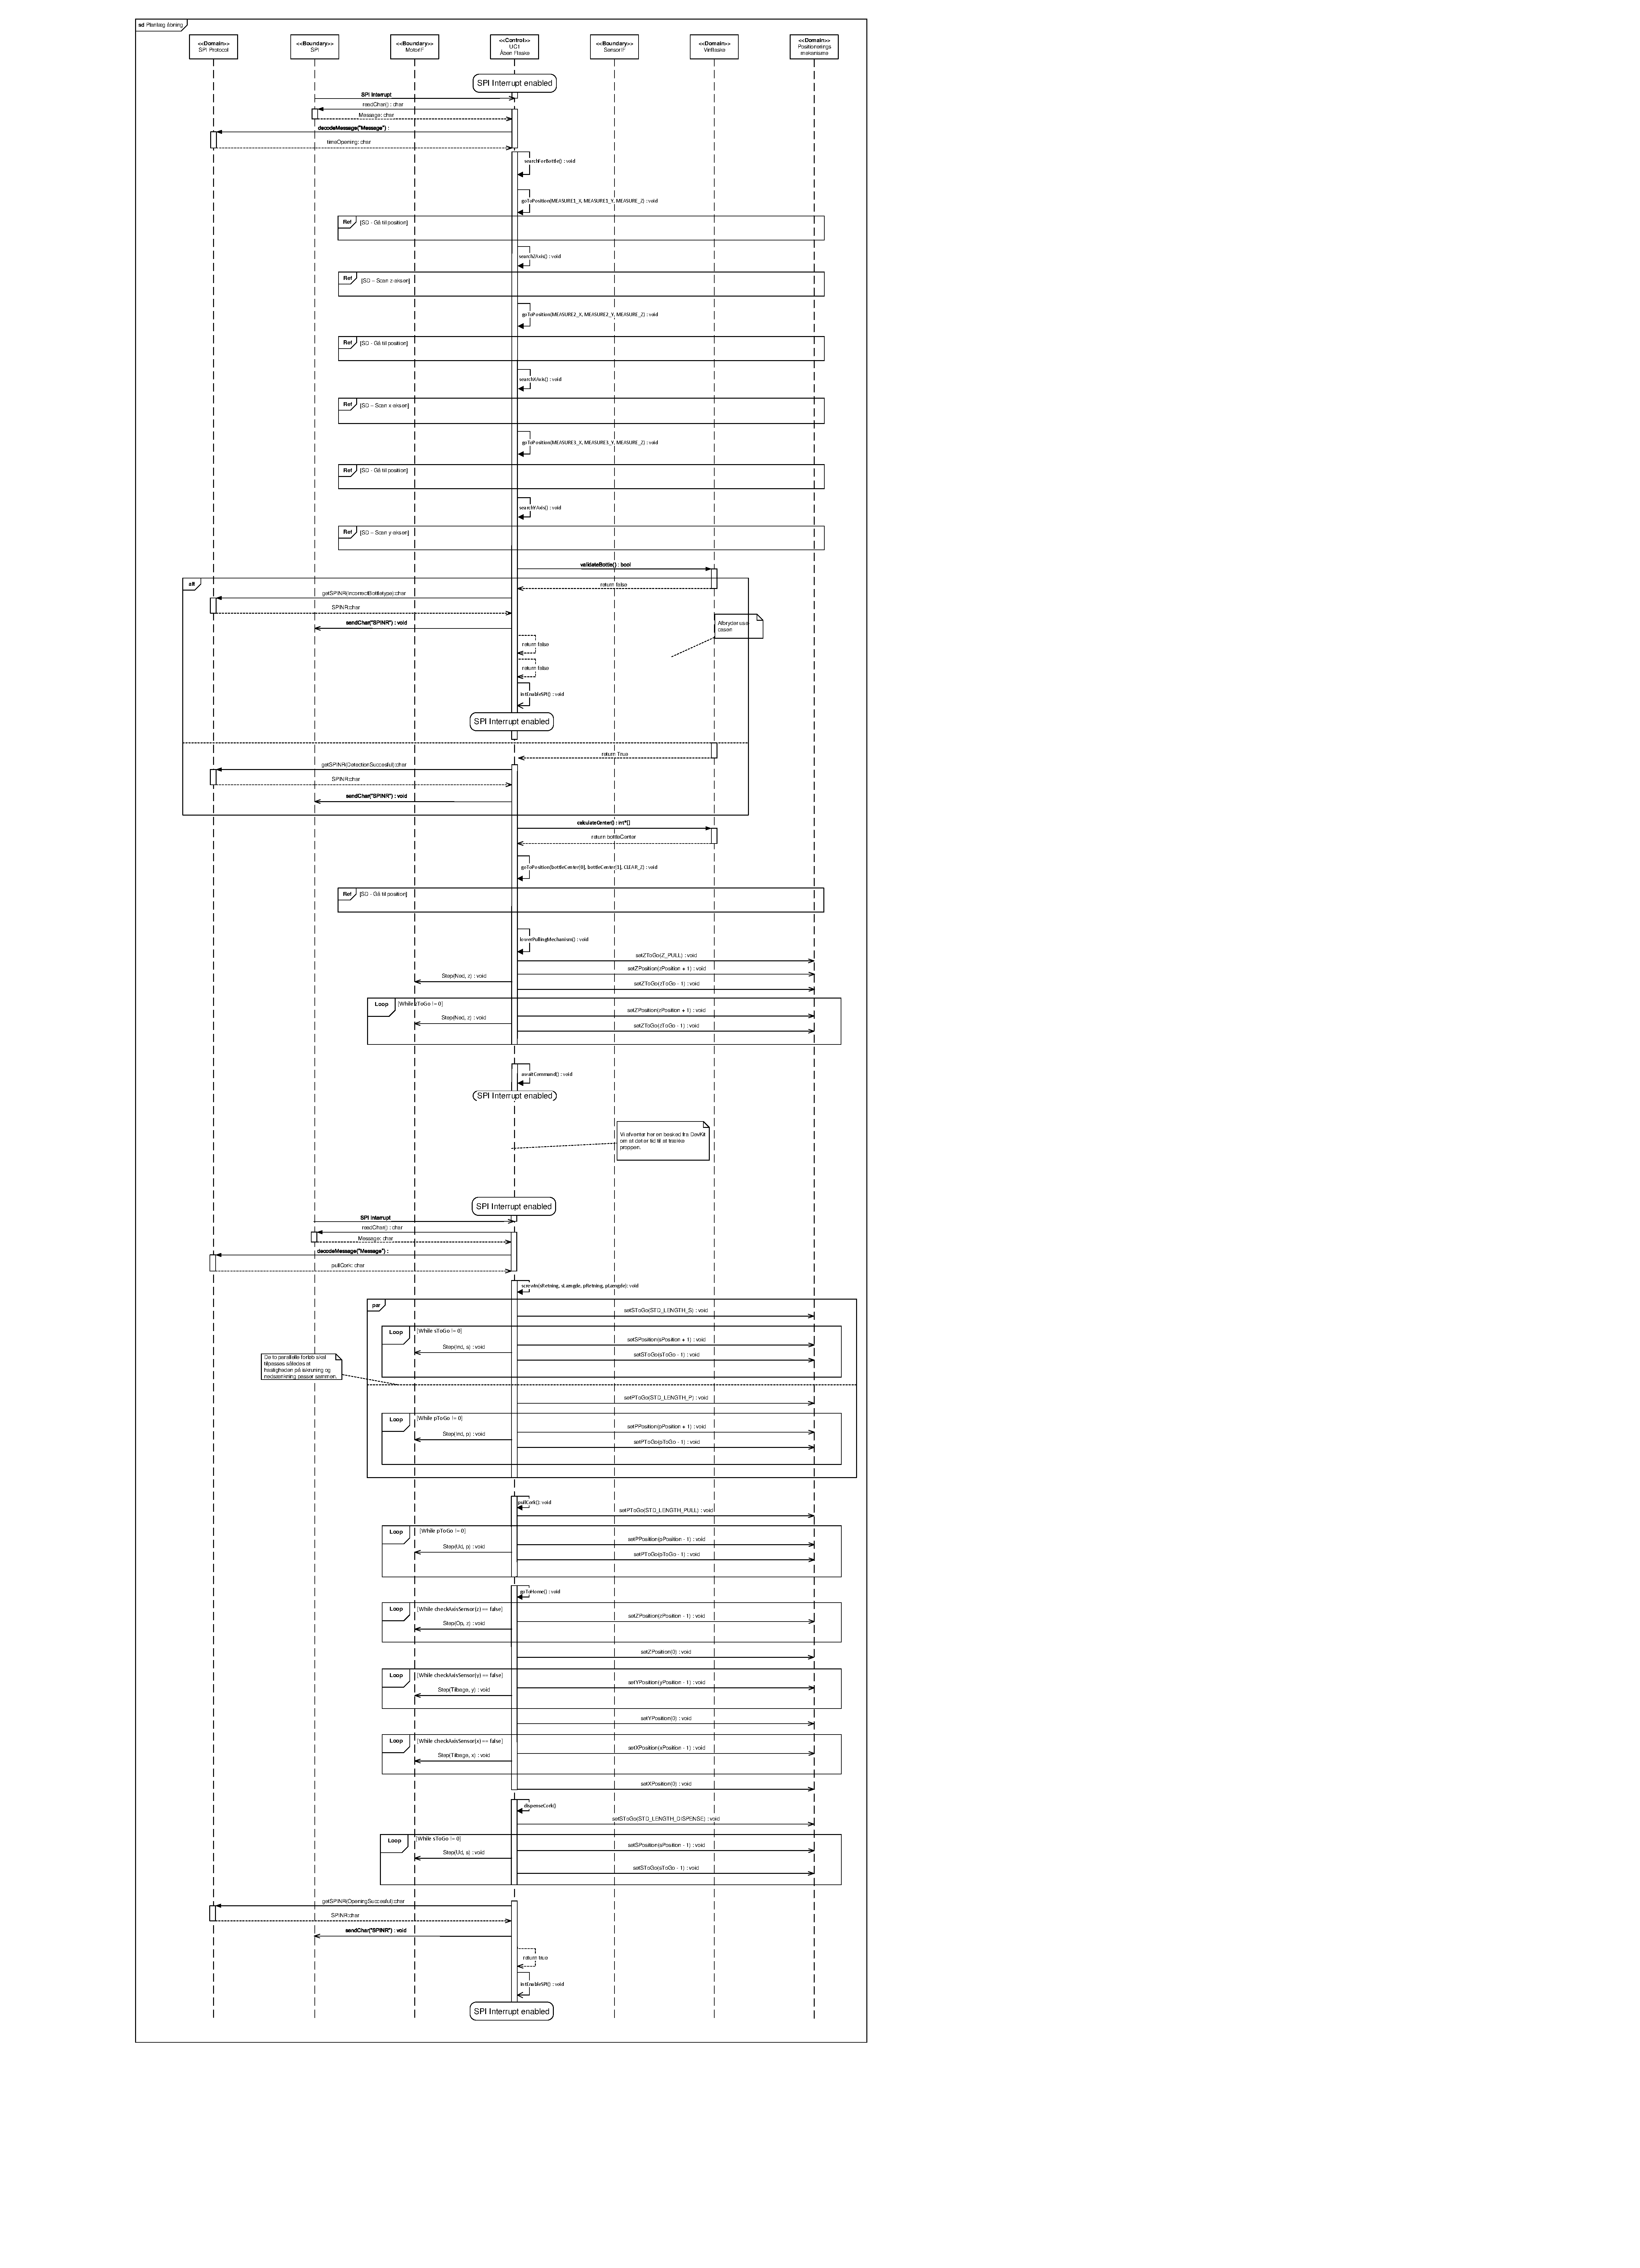
\includegraphics[scale=0.18,trim=0 0 0 0, clip]{APPSoC/UC2-planlaeg-aabning-v1-simplified}
\end{figure}

Ud fra sekvensdiagrammet på figur \ref{SD:PSoC:UC2} side \pageref{SD:PSoC:UC2} samt sekvensdiagrammerne sektionen "Sekvensdiagrammer der anvendes i Applikationsmodel for use-case 1 og 2" er der udført metodeidentifikation hvilket har resulteret i klassediagrammet på figur \ref{CD:PSoC:UC2} side \pageref{CD:PSoC:UC2}.

\begin{figure}[H]
	\caption{Klassediagram for use-case 2: Planlæg åbning}
	\label{CD:PSoC:UC2}
	\includegraphics[scale=0.35,trim=0 0 0 0, clip]{APPSoC/UC2-CD-planlaeg-aabning-PSoC}
\end{figure}
